\documentclass[
12pt, paper=a4,  listof=totocnumbered, % lists are also included in table of contents
, % Don't add a period at the end of a chapter number
]{scrreprt}

\usepackage{chngcntr}
    \counterwithout{footnote}{chapter}
    \counterwithout{figure}{chapter}

% get custom bibliography style working without prepending [brackets]
\usepackage{natbib}

%\setcitestyle{aysep={}} % remove comma as delimiter 

% breaks line at hyphens (resolves formatting issues in bibliography)
\usepackage[hyphens]{url}


% if you insist on Arial... then uncomment the following
\usepackage{helvet}
\renewcommand{\familydefault}{\sfdefault}

\usepackage[left=2.5cm,right=2.5cm,top=2.5cm,bottom=2.5cm]{geometry} % margins
%\addtolength{\footskip}{-0.7cm}% foot larger by 0,7 cm  (Raises the page number)


%\usepackage[onehalfspacing]{setspace} % line space 1,5
\usepackage[doublespacing]{setspace}
%\doublespacing

%\setlength{\parindent}{12pt} % Indent at start of paragraphs  6pt

\usepackage[utf8]{inputenc} %UTF-8 to encode many characters => for many characters, you can just input the character and avoid a macro

\usepackage[english]{babel} % english hyphenations
%\usepackage[T1]{fontenc} %wichtig für Trennung von Wörtern mit Umlauten
\usepackage{microtype} % align margins

% for multi line comments
\usepackage{comment}

\usepackage{graphicx} % import graphics
\usepackage{placeins}% places the graphics within text

% Abbreviation's directory
% printonlyused - only if used
% withpage - the first occurrence's page number is listed too
\usepackage[withpage]{acronym}

% for tables
\usepackage{longtable}
\usepackage[table]{xcolor}
\usepackage{multirow}


\usepackage[hidelinks]{hyperref} %https://tex.stackexchange.com/questions/823/remove-ugly-borders-around-clickable-cross-references-and-hyperlinks

%for chapter spaces
\begin{document}

%\renewcommand{\thechapter}{\Roman{chapter}}
%TITELBLATT:!!!!!!!!!!!!!!!!!!!!!!!!!!!!!!!!!!!!!!!!!!!!!!!!!!!!!!!!!!!!!!!!!!!!!!!!!!!!!!!!!!!!!!!!!!!!!

\label{titlePage}
\begin{figure}[h]
\centering

\includegraphics[width=0.50\textwidth]{pics/logo.pdf}
\end{figure}
\FloatBarrier

\begin{Large} 
\begin{center}
Network Security
\end{center}
\end{Large} 

\vspace*{5mm}

\begin{large} 
\begin{center}
University of Essex
\end{center}
\end{large} 

\begin{large} 
\begin{center}
Study-branch: MSc. Cyber Security
\end{center}
\end{large}



\begin{Large} 
\begin{center}
\textbf{Vulnerability Audit and Assessment - Executive Summary}
\end{center}
\end{Large}

\vspace*{5mm}

\begin{large} 
\begin{center}
Advisor: Beran Necat
\end{center}
\end{large} 




\pagestyle{empty} % no page numbering on the cover



\renewcommand{\thechapter}{\Roman{chapter}}

\pagestyle{plain}

\pagenumbering{Roman} %the intro is counted with roman numbers
\setcounter{page}{2} %starting with page 2 (page 1 is the titel)

\tableofcontents %table of contents
\listoffigures %List of figures
\listoftables %list of tables

%% Abbreviations list
\renewcommand\refname{Abbreviations} \chapter{Abbreviations}
% The abbreviations list should contain all abbreviations that are not common-knowledge.
\begin{acronym}[NMWC] % the longest abbreviation here (for layout)
    \setlength {\itemsep}{-\parsep} % geringerer Zeilenabstand    	 

    \acro{CMS}{Content-Management System}
    

\end{acronym}

% Acronyms should be made hyperreffed the first time they appear in text with
% \ac{CI}  

\renewcommand{\thechapter}{\arabic{chapter}} %Count chapters with arabic numbers and not roman numbers
\setcounter{chapter}{0} %Reset chapter counter
\pagenumbering{arabic}

\chapter{Summary of the Scope}
The scope comprised the examination of the network resources and vulnerabilities present in the web application. The resources were assessed using the following angles of attack:
\begin{itemize}
    \item As an external user with no access to internal network resources. This approach is taken to assess the application from the perspective of a genuine hacker with no prior information about the system.
    \item As an external website visitor using the browser without admin access. This approach is taken to observe some risks that can be observed visually from the CMS sites.
\end{itemize}
The testing was performed manually using a VM Kali Linux, and the tools installed, as the IP used for testing is not whitelisted; there is a possibility of getting blocked during the assessment.

\newline
\begin{table}[h!]
\centering
\begin{tabular}{||c| c||} 
 \hline
 CIDR BLOCK & IP  \\ [0.5ex] 
 \hline
 /32 & 68.66.247.187  \\
 \hline
\end{tabular}
\caption{IP block tested}
\label{table:1}
\end{table}

\chapter{Limitations}
The assessment consisted of a few constraints as the project.  The following limitations were encountered during the vulnerability assessment.
\begin{enumerate}
    \item Evaluating against the frameworks, the points requiring internal organizational knowledge could not be verified, i.e., backups exist, data encryption at rest, and the presence of Logs and SIEM. Therefore the system could not be evaluated completely 
    \item On-site assessments could not be done, as the data centers are physically out of reach for us.
    \item All intrusive testing,i.e., SQL injections and malware uploads, to verify the exploits could not be carried out, as there are no legal permissions to carry out such tests.
    \item Ping-based tests are avoided, as the site is a shared hosting consisting of other CMS sites with the IP, which would not bring any more useful information.
\end{enumerate}
\chapter{Analysis}
\section{Summary of the Scope}
The scope comprised the examination of the network resources and vulnerabilities present in the web application. The resources were assessed using the following angles of attack:
\begin{itemize}
    \item As an external user with no access to internal network resources. This approach is taken to assess the application from the perspective of a genuine hacker with no prior information about the system.
    \item As an external website visitor using the browser without admin access. This approach is taken to observe some risks that can be observed visually from the CMS sites.
\end{itemize}

\section{Threat Modeling}
Threat modeling is a technique that allows us to detect and address top threats that can have a significant impact on the application \citep{threat_modeling}, also used in this assessment. The threats in the table will be tested against the system to detect any vulnerabilities.
Using the DFD (see figure \ref{fig:dfd}), we can list some threats utilizing the model.

\begingroup
\centering
\setlength{\tabcolsep}{6.5pt} % Default value: 6pt
\renewcommand{\arraystretch}{1.8} % Default value: 1
\begin{longtable}{ |p{7cm}| p{8cm} |}
\caption{STRIDE Modeling}
    \label{table:spoofing}
\hline
\rowcolor{grey!15}
\textbf{STRIDE} & \textbf{Threats}\\
\hline
Spoofing & 
\vspace{-\baselineskip}
\begin{enumerate}
    \item DNS spoofing allowing to redirect to a malicious site.
    \item Ip Spoofing \citep[p.~2]{ip_spoofing}
\end{enumerate} \\
\hline
Tampering & 
\vspace{-\baselineskip}
\begin{enumerate}
    \item Upload malicious files.
    \item Cross-Site Request Forgery. \citep[p.~538]{crsf}
\end{enumerate} \\
\hline
Repudiation & 
\vspace{-\baselineskip}
\begin{enumerate}
    \item Malicious activities are not tracked.
\end{enumerate} \\
\hline
Information Disclosure & 
\vspace{-\baselineskip}
\begin{enumerate}
    \item SQL Injection into the database.
    \item Various network information is public.
\end{enumerate} \\
\hline
Denial of Service & 
\vspace{-\baselineskip}
\begin{enumerate}
    \item The CMS site is hit with a DoS attack.
\end{enumerate} \\
\hline
Elevation of Privileges & 
\vspace{-\baselineskip}
\begin{enumerate}
    \item Unauthorized users with admin privileges are added.
\end{enumerate} \\
\hline
\end{longtable}
\endgroup

\begin{figure}[h!]
\centering
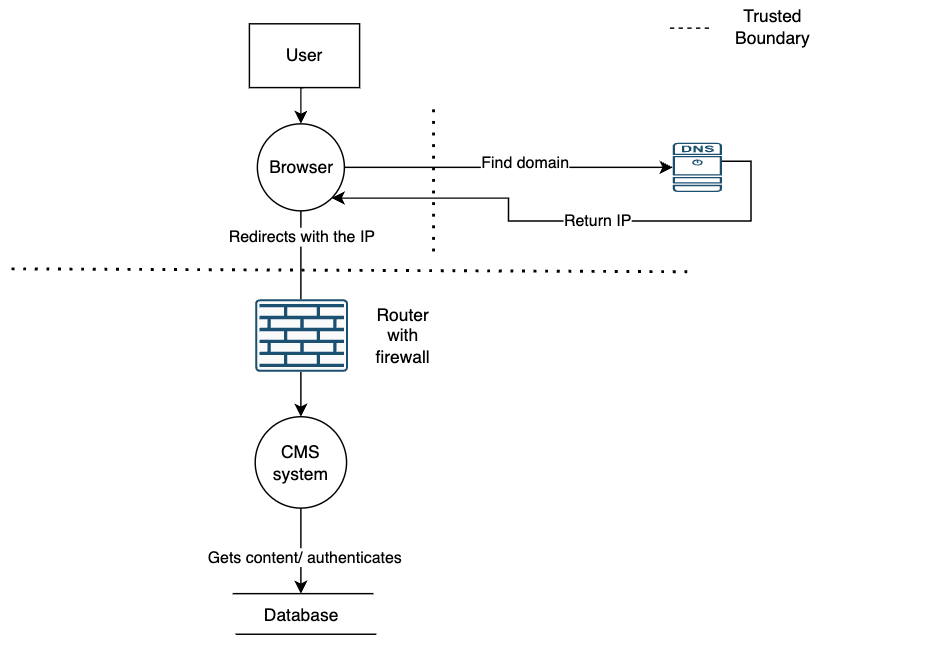
\includegraphics[width=\textwidth, height=420px]{pics/dfd.png}
\caption{DFD level 0 for the CMS system}\label{fig:dfd}
\end{figure}


\section{Vulnerability Assessment}
For the vulnerability assessment, the automated tools (see table \ref{table:tools}) mentioned in the baseline analysis were used to scan for known threats using the adversary behaviors defined in MITRE Enterprise ATT\&CK matrix \citep[p.~158]{xiong2022cyber}.

\begin{comment}
Additionally, the assessment and reconnaissance are performed using the MITRE Enterprise ATT\&CK matrix \citep{mitre_url}, as this model describes the adversary behaviors that measure the system's resilience at an enterprise level \citep[p.~158]{xiong2022cyber}.
\end{comment}



\begingroup
\centering
\setlength{\tabcolsep}{6.5pt} % Default value: 6pt
\renewcommand{\arraystretch}{1.8} % Default value: 1
\begin{longtable}{ |p{5cm}| p{10cm} |}
\caption{Results from the tools used in the assessment}
    \label{table:tools}
\hline
\rowcolor{grey!15}
\textbf{Tool}  & \textbf{Result}\\
\hline
Metasploit \& Nmap &  
\vspace{-\baselineskip}
\begin{enumerate}
    \item Discovered network misconfigurations.
    \item SSL/TLS scans were carried out for the open ports.
    \item Tested against major CRM threats (i.e., SQL injection, XSS, RCE, Directory traversal).
    \item Wordlist scans for discovering vulnerable paths were executed.
\end{enumerate}\\
\hline
Cmsmap &  
\vspace{-\baselineskip}
\begin{enumerate}
    \item CMS and PHP version was scanned and its vulnerabilities.
\end{enumerate}\\
\hline
DNSrecon &  
\vspace{-\baselineskip}
\begin{enumerate}
    \item Performed reverse lookup and CDN detection.
    \item Performed DNS Zone transfer \citep[p.~193]{zone_transfer}.
    \item Performed Cache Snooping and DNS Recursion.
    \item Performed Zone walking.
\end{enumerate}\\
\hline
\end{longtable}
\endgroup

\section{GDPR Analysis}
Using the GDPR compliance checklist, the website is evaluated for compliance with GDPR \citep{gdpr_checklist}. Failure to comply with GDPR rules with severe violations can be fined up to 4\% of the total turnover, or €20 million \citep[p.~32]{eu_fines}. Table \ref{table:gdpr} summarizes the discovered GDPR compliance results for the CMS system.


\begingroup
\centering
\setlength{\tabcolsep}{6.5pt} % Default value: 6pt
\renewcommand{\arraystretch}{1.8} % Default value: 1
\begin{longtable}{ |p{3cm}|p{5cm}| p{7cm} |}
\caption{GDPR Assessment}
    \label{table:gdpr}
\hline
\rowcolor{grey!15}
\textbf{Article GDPR} & \textbf{Name}  & \textbf{Status}\\
\hline
Art.3 & Representative of Controller in the European Union  &
\vspace{-\baselineskip}
\begin{enumerate}
    \item A representative in the European Union is required as the CRM is hosted in the United States and processes personal data, which is unknown.
\end{enumerate}\\
\hline
Art.12 & Transparent privacy policy use, with the subject's consent.  &  
\vspace{-\baselineskip}
\begin{enumerate}
    \item A consent layer for informing users of the information the cookies collect is missing.
    \item Granular consent is also not present.
    \item Privacy policy of the website link is not present.
\end{enumerate}\\
\hline
Art.25 & Data Protection by Design and default.  &  
The databases containing personal data are available on the public internet, creating a risk of personal data breaches.\\
\hline
Art.33 \& 34 & Notification of breaches.  &  
 Logging and monitoring to detect unusual behaviors are required but cannot be confirmed.
\\
\hline
Art.38 & Presence of Data Protection Officer.  &  
 A data protection officer handling critical breach incidents is required. The availability of the DPO is unknown.
\\
\hline
Art.32 & Security of Processing.  &  
\vspace{-\baselineskip}
\begin{enumerate}
    \item Unencrypted email servers with ports (110, 143, 465, 587, and 2525) are used and are susceptible to man-in-the- middle-attacks.
    \item The CRM website uses TLS-encrypted connections for data exchange. Unencrypted ports, i.e., 80 and 8080, are redirected to encrypted ones.  
\end{enumerate}\\
\hline
\end{longtable}
\endgroup
After evaluating the CMS system with the GDPR directive (see Table \ref{table:gdpr}), it can be concluded that significant shortcomings are present in the system, which break the GDPR directive, as many required features like privacy policy, cookie consent, data protection are not adequately implemented and the company can be fined for not them.

\section{CIS Analysis}
%An evaluation of the CIS v8 framework is a set of recommended actions to prevent common attacks on networks and systems. 
An evaluation of the CIS v8 framework is chosen as it prioritizes a simple list of steps in comparison to other frameworks, which can be easily implemented also by small and medium-sized organizations with a low budget \citep[p.~59]{CIS}. Table \ref{table:cis} summarizes the evident shortcomings of the system according to the CIS control safeguards.

\begin{comment}
    
    \begin{figure}[h!]
    \centering
    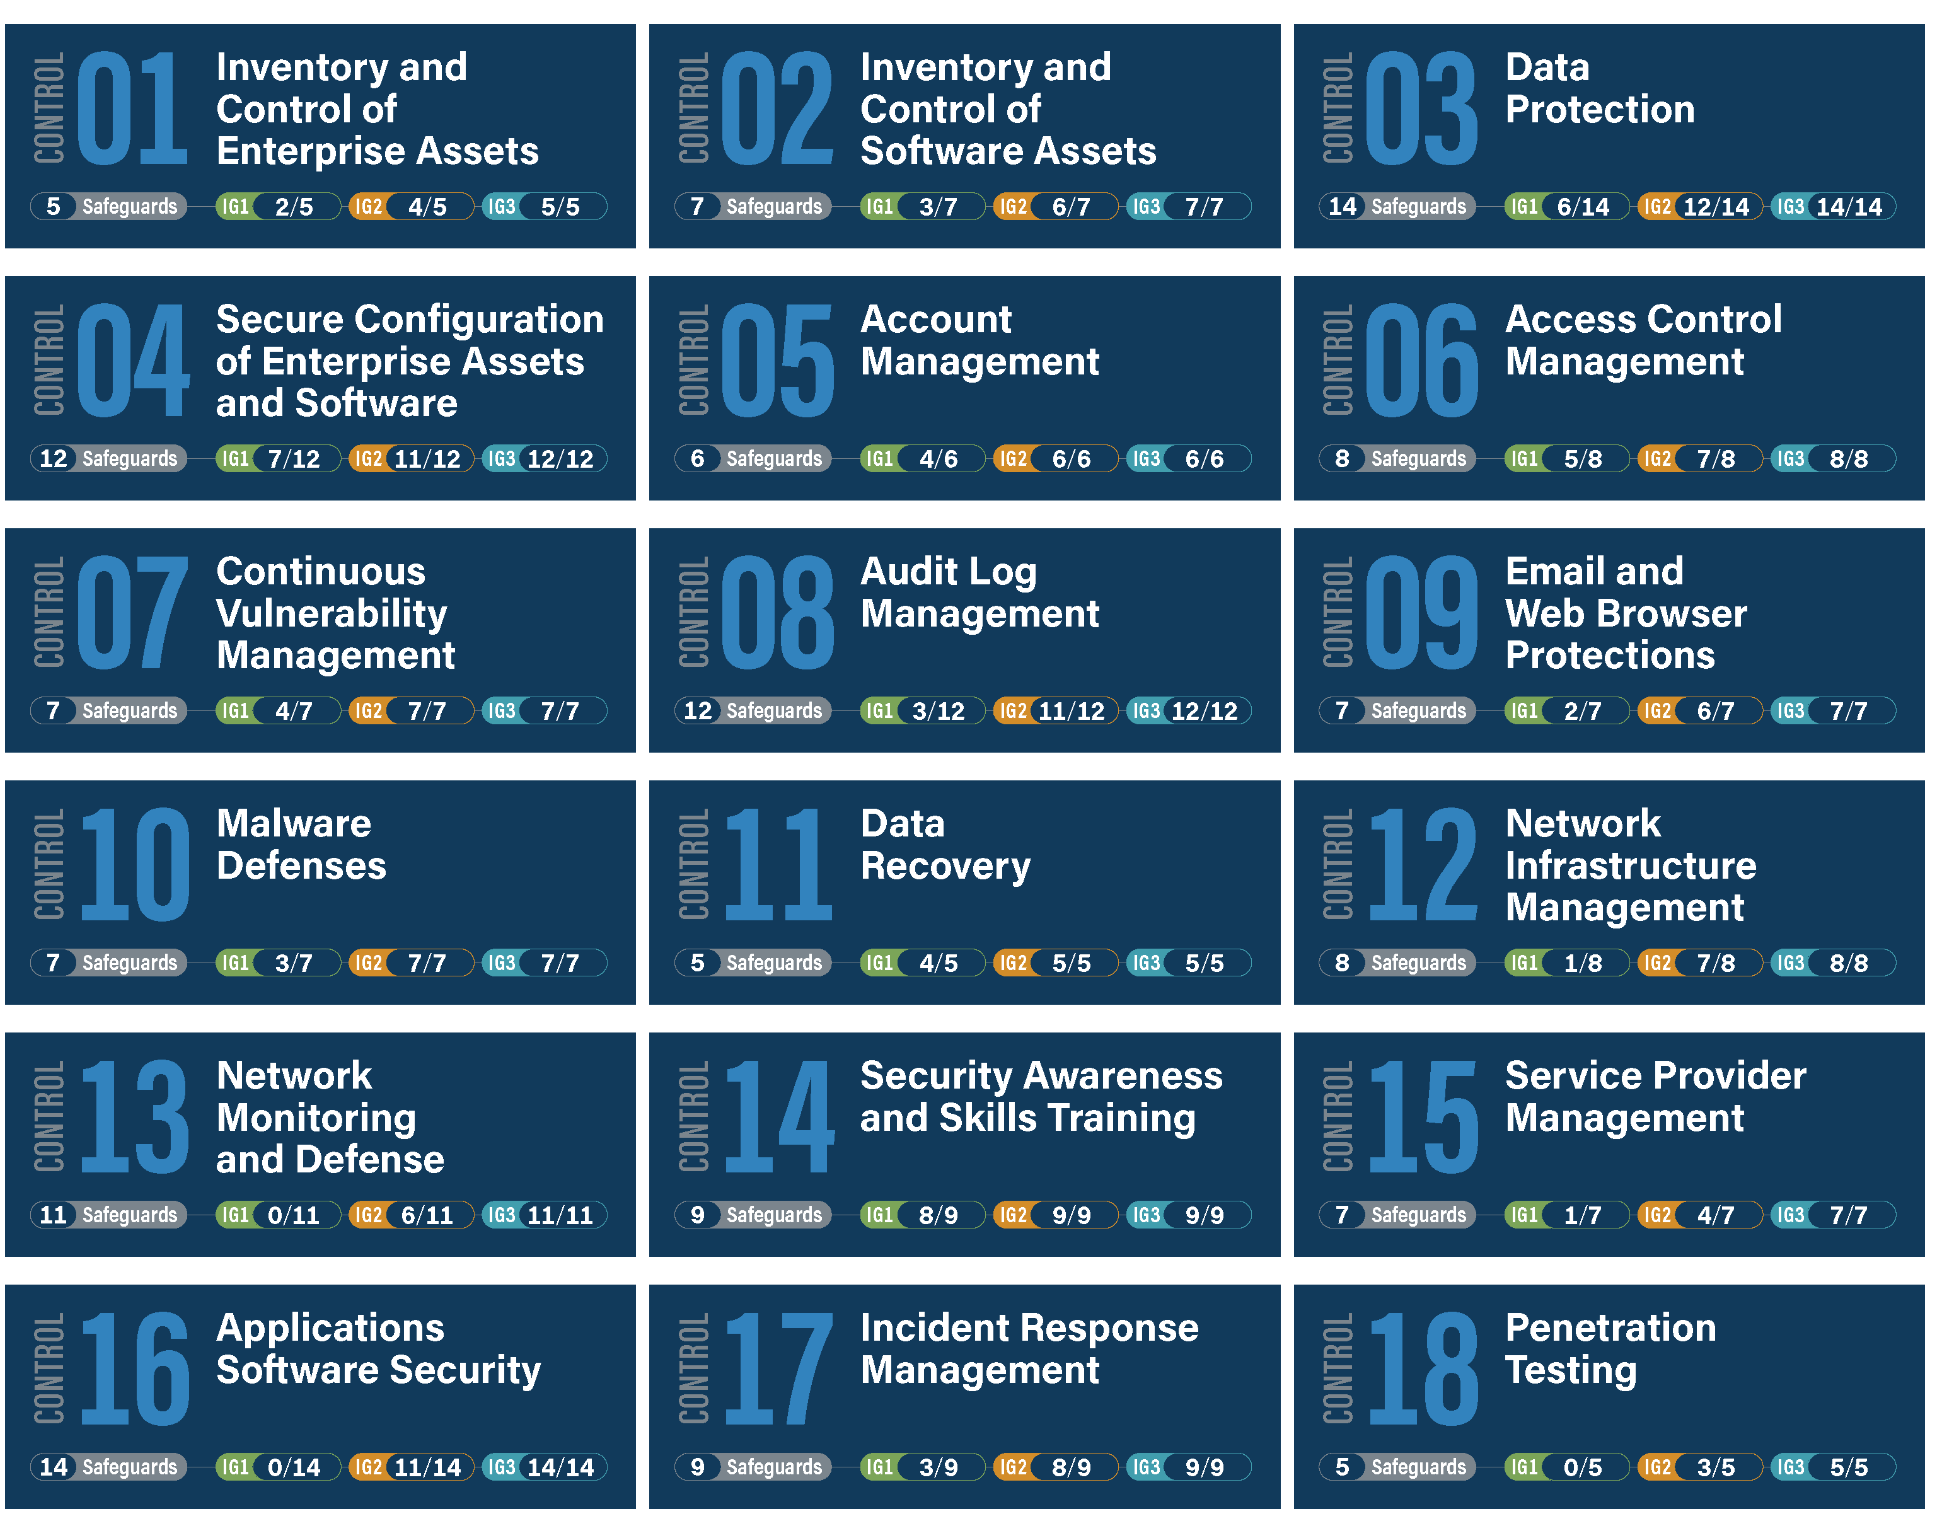
\includegraphics[width=\textwidth]{pics/cis_steps.png}
    \caption{(source:https://www.cisecurity.org/controls/implementation-groups/ig3) CIS Controls}\label{fig:bar_risks}
    \end{figure}

\end{comment}

\newpage
\begingroup
\centering
\setlength{\tabcolsep}{6.5pt} % Default value: 6pt
\renewcommand{\arraystretch}{1.8} % Default value: 1
\begin{longtable}{ |p{7cm}| p{8cm} |}
\caption{CIS Controls}
    \label{table:cis}
\hline
\rowcolor{grey!15}
\textbf{CIS Control}  & \textbf{Status}\\
\hline
Inventory and Control of Enterprise Assets  &  
 Unauthorized assets like databases and FTP servers are not checked regularly, as they are open to the public.\\
\hline
Inventory and Control of Software Assets  &  
Not all software components, i.e., DNS servers and databases, are up-to-date.
\\
\hline
Data Protection  &  
Mail and FTP servers do not use encryption in transit.\\
\hline
Network Infrastructure Management  &  
 Network infrastructure is not up-to-date, i.e., the DNS server is outdated and contains many vulnerabilities.\\
\hline
\end{longtable}
\endgroup

\section{Limitations}
The assessment consisted of a few constraints as the project. The following limitations were encountered during the vulnerability assessment.
\begin{enumerate}
    \item Evaluating against the frameworks, the points requiring internal organizational knowledge could not be verified, i.e., backups exist, data encryption at rest, the presence of Logs and SIEM, presence of data protection officers. Herefore, the system could only be evaluated partially. 
    \item Some GDPR articles concerning Right to Access, Correct, and Erase Data cannot be evaluated, as we do not have access to any valid user. 
    \item On-site assessments could not be done, as the data centers are physically out of reach for us.
    \item All intrusive testing to verify the found exploits could not be carried out, as there are no legal permissions to attack the system, leading to only assumptions about the blast radius of the vulnerabilities.
\end{enumerate}





\section{Findings}
Testing discovered 9 key issues in the system according to business risk, and Figure \ref{fig:bar_rankings} depicts the total number of cases according to their order.

\newline
\begin{figure}[h!]
\centering
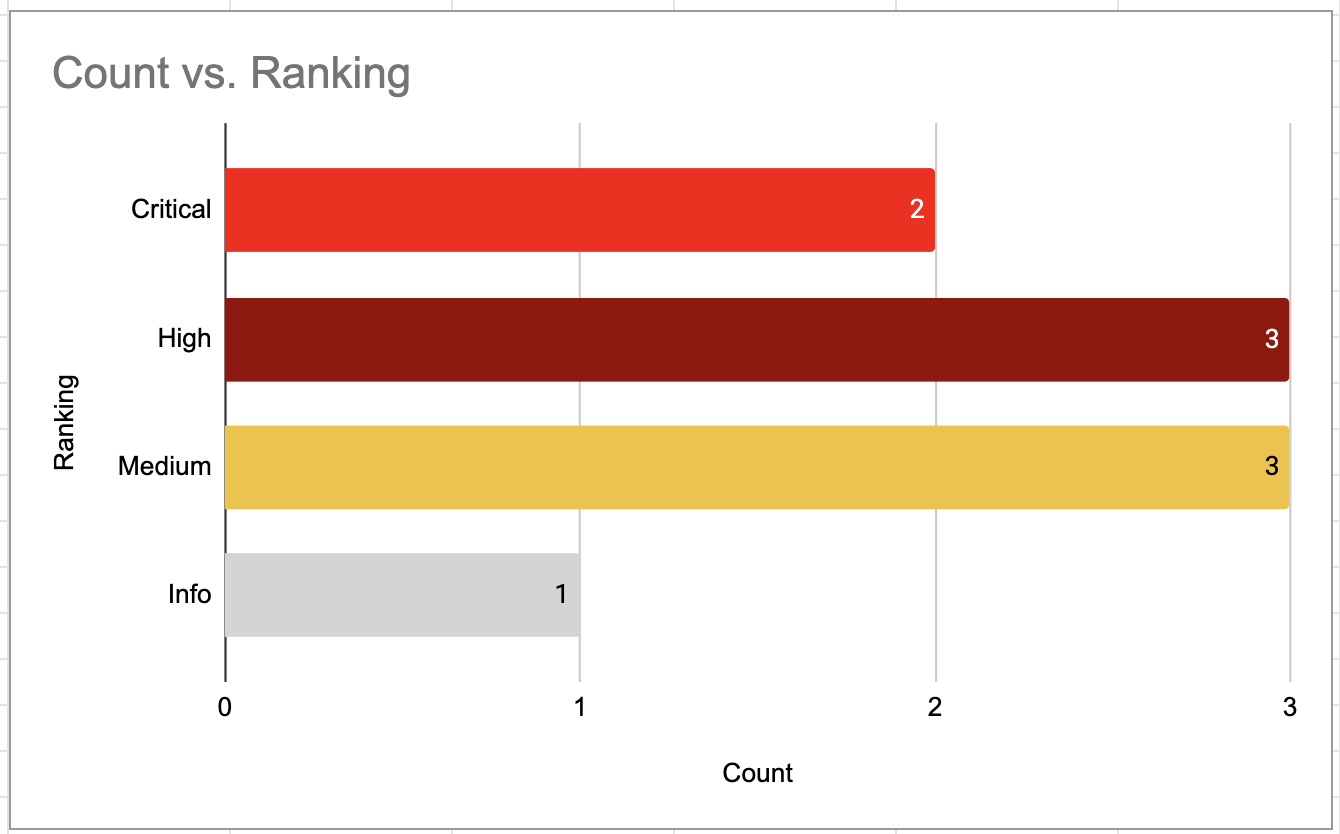
\includegraphics[width=\textwidth, height=350px]{pics/rankings.png}
\caption{Distribution of risks}\label{fig:bar_rankings}
\end{figure}


\newpage
\section{Key Findings}

List of security threats found in comparison to the baseline analysis are listed below:

\begin{enumerate}
    \item Phishing and social engineering of the mail servers.
    \item Denial of service due to some CVEs in the old database versions and mitigations like CDN also not present.
    \item Cross-Site Scripting as headers are not implemented in the CMS site.
    \item Security misconfigurations as many ports are made public unnecessarily.
    \item Ransomware attacks can be carried out with more ease, as important data-stores are open in public.
\end{enumerate}

\begin{comment}
   \begin{figure}[htp!]
\centering
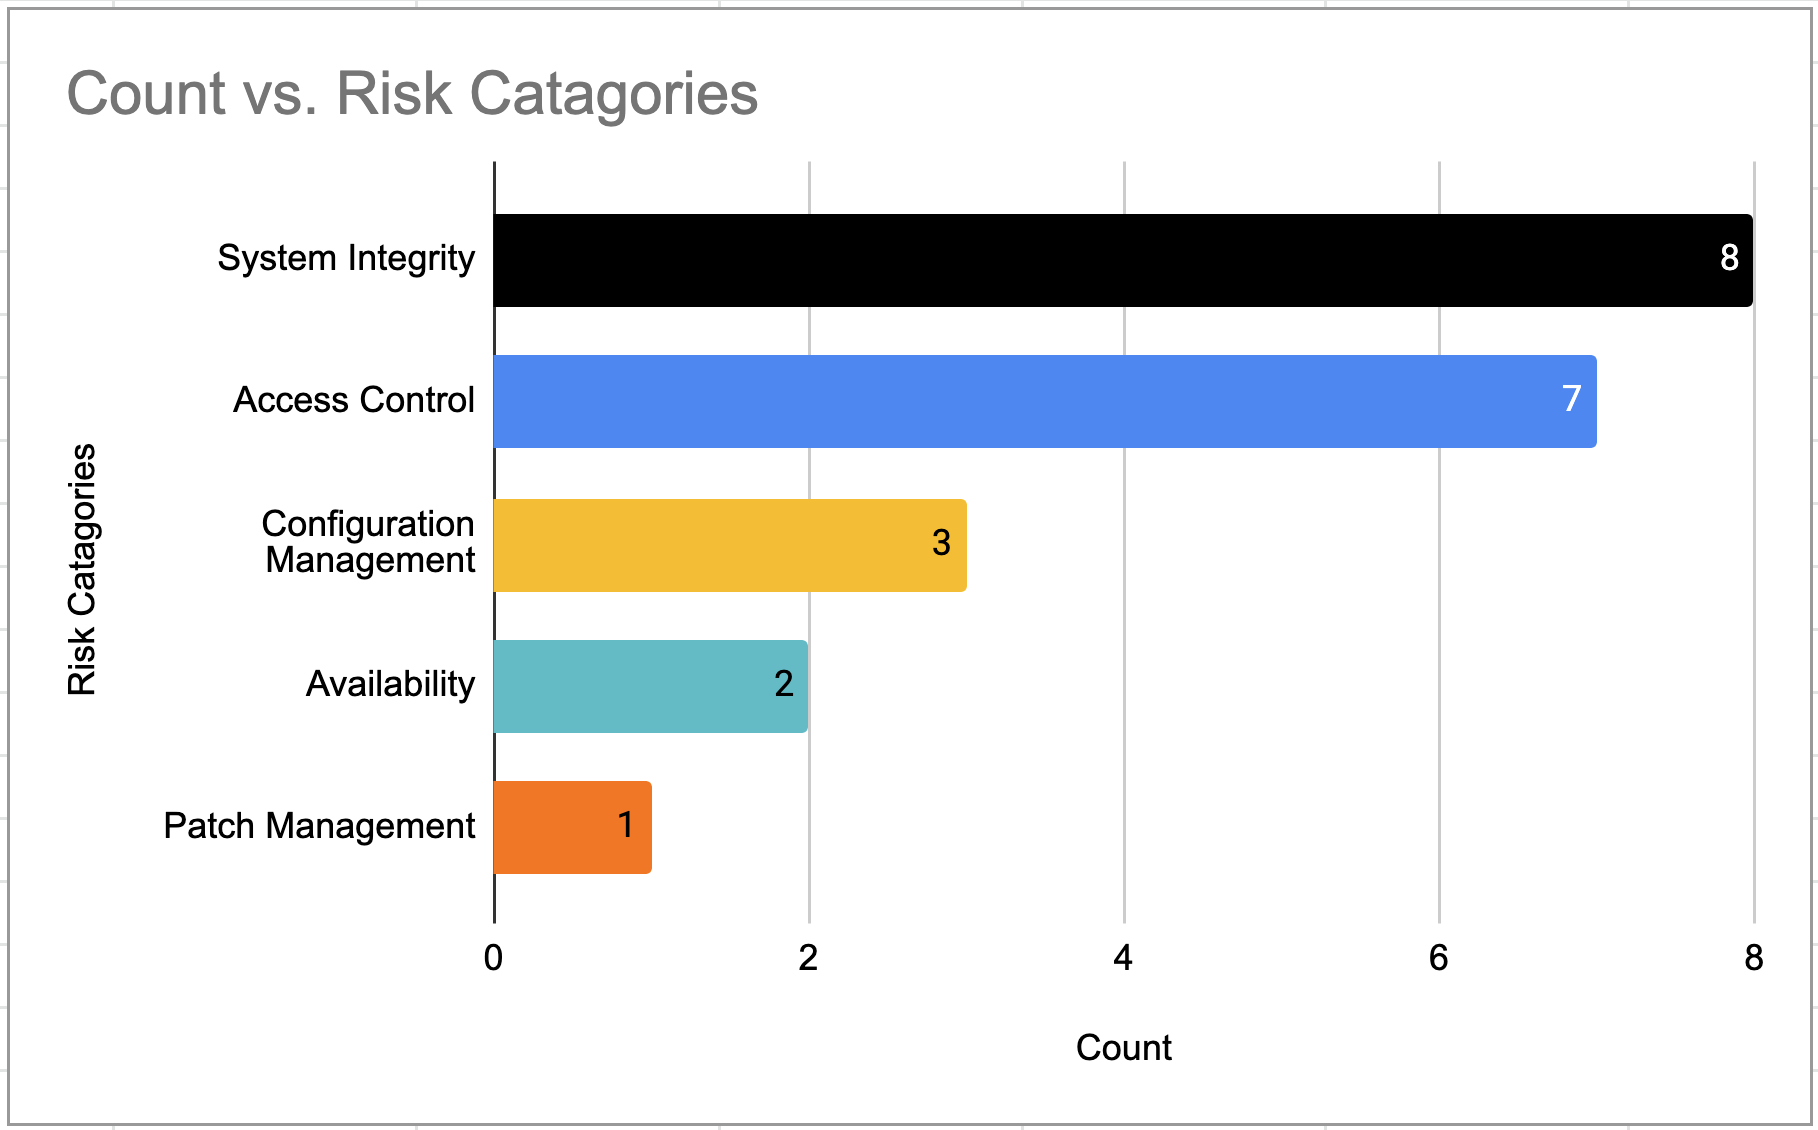
\includegraphics[width=\textwidth, height=330px]{pics/risk_cat.png}
\caption{Risk Catagories Count}\label{fig:bar_risks}
\end{figure} 
\end{comment}


\begingroup
\centering
\setlength{\tabcolsep}{6.5pt} % Default value: 6pt
\renewcommand{\arraystretch}{1.8} % Default value: 1
\begin{longtable}{ |p{1.5cm}| p{6cm}|p{6.3cm}|}
\caption{Key Findings ordered by Priority}
    \label{table:key_findings}
\hline
\rowcolor{grey!15}
\textbf{Risk}  & \textbf{Finding}& \textbf{Recommendation}\\
\hline
\cellcolor{red!95} Critical  & Externally exposed Network Resources, i.e., databases, FTP, DNS servers. Information theft and DoS attacks can be performed with less effort.
 & Ports 21, 3306, and 5432 should be closed from the public internet as they are not necessary to be open for running the CMS. %CDN should be used to relieve the load on the servers.
\\
\hline
\cellcolor{red!95} Critical  & Privacy policy and cookie confirmation for users not available, therefore breaking GDPR directive. & A detailed cookie consent form and privacy policy, that a user can explicitly confirm to use the site should be implemented \citep[p.~2]{godr_cookie}.
\\
\hline
\cellcolor{red!55} High  & Insecure database versions  containing multiple CVEs. This can lead to personal data theft.
 & The vulnerable versions of the database must be updated to a secure one. In addition, regular security automatic scans with dynamic and static application testing should be carried out.
\\
\hline
\cellcolor{red!55} High  & Mail servers are unencrypted and could be intercepted, leading to a leak of sensitive information. & The mail servers should use TLSv1.3 to encrypt the traffic from getting intercepted during transit.\citep[p.~10]{tls_smtp}. 
\\
\hline
\cellcolor{red!55} High  & Malicious Code injection possible(XSS, CSRF forgery) & The HTML inputs should be sanitized, set Content-security policy header, and CSRF tokens \citep[p.~75]{xss_crsf}.
\\
\hline
\cellcolor{yellow!95} Medium  & Ip spoofing, DNS server spoofing, and Cache Poisoning possible.
& Implement DNSSEC to protect the integrity of the server and turn off DNS recursion in the Bind server. \citep[p.~38]{guo2006spoof}
\\
\hline
\cellcolor{yellow!95} Medium  & Server and application version is public.& Do not make server and application versions public information.
\\
\hline
\cellcolor{yellow!95} Medium  & DNS server is outdated and can cause an outage of the service because of present vulnerabilities..& Update DNS bind to v9.18.12.
\\
\hline
\cellcolor{grey!55} Info  & Mail server is not protected against spam and phishing.& A DMARC record in the DNS for the mail server should be included, which can validate the emails are from a genuine sender \citep[p.~7]{dmarc}.
\\
\hline
\end{longtable}
\endgroup

\section{Conclusion}
Looking at table \ref{table:key_findings}, it can be concluded that the CMS system has severe critical flaws such as non-GDPR compliance because of missing privacy policies and consent, databases that might contain sensitive personal data are with open ports in the public internet. These errors pose a significant danger to the security operations of the system from attackers. Additionally, since the system is not GDPR conform, therefore is liable to be fined for not imposing the required elements. Herefore, the website is not production ready without resolving the high and critical issues from the findings.

\appendix 

% ---- Bibliography ----
%
% BibTeX users should specify bibliography style 
% References will then be sorted and formatted in the correct style.
%
 %\bibliographystyle{alpha}
\renewcommand{\bibname}{References}
\bibliographystyle{agsm}
\bibliography{biblio}

\end{document}
